%%%%%%%%%%%%%%%%%%%%%%%%%%%%%%%%%%%%%%%%%%%%%%%%%%%%%%%%%%%%%%%%%%
%%%%%%%%%%%%%%%%%%%%%%%%%%%%%%%%%%%%%%%%%%%%%%%%%%%%%%%%%%%%%%%%%%
%Packages
\documentclass[10pt, a4paper]{article}
\usepackage[top=3cm, bottom=4cm, left=3.5cm, right=3.5cm]{geometry}
\usepackage{amsmath,amsthm,amsfonts,amssymb,amscd, fancyhdr, color, comment, graphicx, environ}
\usepackage{float}
\usepackage{mathrsfs}
\usepackage[math-style=ISO]{unicode-math}
\setmathfont{TeX Gyre Termes Math}
\usepackage{lastpage}
\usepackage[dvipsnames]{xcolor}
\usepackage[framemethod=TikZ]{mdframed}
\usepackage{enumerate}
\usepackage[shortlabels]{enumitem}
\usepackage{fancyhdr}
\usepackage{indentfirst}
\usepackage{listings}
\usepackage{sectsty}
\usepackage{thmtools}
\usepackage{shadethm}
\usepackage{hyperref}
\usepackage{setspace}
\hypersetup{
    colorlinks=true,
    linkcolor=blue,
    filecolor=magenta,      
    urlcolor=blue,
}
%%%%%%%%%%%%%%%%%%%%%%%%%%%%%%%%%%%%%%%%%%%%%%%%%%%%%%%%%%%%%%%%%%
%%%%%%%%%%%%%%%%%%%%%%%%%%%%%%%%%%%%%%%%%%%%%%%%%%%%%%%%%%%%%%%%%%
%Environment setup
\mdfsetup{skipabove=\topskip,skipbelow=\topskip}
\newrobustcmd\ExampleText{%
An \textit{inhomogeneous linear} differential equation has the form
\begin{align}
L[v ] = f,
\end{align}
where $L$ is a linear differential operator, $v$ is the dependent
variable, and $f$ is a given non−zero function of the independent
variables alone.
}
\mdfdefinestyle{theoremstyle}{%
linecolor=black,linewidth=1pt,%
frametitlerule=true,%
frametitlebackgroundcolor=gray!20,
innertopmargin=\topskip,
}
\mdtheorem[style=theoremstyle]{term}{Terminologies}
\newenvironment{Solution}{\textbf{Solution.}}

\definecolor{codegreen}{rgb}{0,0.6,0}
\definecolor{codegray}{rgb}{0.5,0.5,0.5}
\definecolor{codepurple}{rgb}{0.58,0,0.82}
\definecolor{backcolour}{rgb}{0.95,0.95,0.92}

\lstdefinestyle{mystyle}{
    backgroundcolor=\color{backcolour},   
    commentstyle=\color{codegreen},
    keywordstyle=\color{magenta},
    numberstyle=\tiny\color{codegray},
    stringstyle=\color{codepurple},
    basicstyle=\ttfamily\footnotesize,
    breakatwhitespace=false,         
    breaklines=true,                 
    captionpos=b,                    
    keepspaces=true,                 
    numbers=left,                    
    numbersep=5pt,                  
    showspaces=false,                
    showstringspaces=false,
    showtabs=false,                  
    tabsize=2
}

\lstset{style=mystyle}
%%%%%%%%%%%%%%%%%%%%%%%%%%%%%%%%%%%%%%%%%%%%%%%%%%%%%%%%%%%%%%%%%%
%%%%%%%%%%%%%%%%%%%%%%%%%%%%%%%%%%%%%%%%%%%%%%%%%%%%%%%%%%%%%%%%%%
%Fill in the appropriate information below
\newcommand{\norm}[1]{\left\lVert#1\right\rVert}     
\newcommand\course{XXXX0000}                            % <-- course name   
\newcommand\hwnumber{0}                                 % <-- homework number
\newcommand\Information{Someone}                        % <-- personal information
%%%%%%%%%%%%%%%%%%%%%%%%%%%%%%%%%%%%%%%%%%%%%%%%%%%%%%%%%%%%%%%%%%
%%%%%%%%%%%%%%%%%%%%%%%%%%%%%%%%%%%%%%%%%%%%%%%%%%%%%%%%%%%%%%%%%%
%Page setup
\pagestyle{fancy}
\headheight 35pt
\lhead{\today}
% \rhead{
\includegraphics[width=2.5cm]{logo-hkust.png}}
\rhead{\href{https://github.com/HackStrix}{github.com/hackstrix}}
\lfoot{}
\pagenumbering{arabic}
\cfoot{\small\thepage}
\rfoot{}
\headsep 1.2em
\renewcommand{\baselinestretch}{1.25}
%%%%%%%%%%%%%%%%%%%%%%%%%%%%%%%%%%%%%%%%%%%%%%%%%%%%%%%%%%%%%%%%%%
%%%%%%%%%%%%%%%%%%%%%%%%%%%%%%%%%%%%%%%%%%%%%%%%%%%%%%%%%%%%%%%%%%
%Add new commands here
\renewcommand{\labelenumi}{\alph{enumi})}
\newcommand{\Z}{\mathbb Z}
\newcommand{\R}{\mathbb R}
\newcommand{\Q}{\mathbb Q}
\newcommand{\NN}{\mathbb N}
\newcommand{\PP}{\mathbb P}
\DeclareMathOperator{\Mod}{Mod} 
\renewcommand\lstlistingname{Algorithm}
\renewcommand\lstlistlistingname{Algorithms}
\def\lstlistingautorefname{Alg.}
\newtheorem*{thm}{Theorem}
\newtheorem*{defn}{Definition}
\newtheorem*{lemma}{Lemma}
\newtheorem*{corol}{Corollary}
\newtheorem{case}{Case}
\newcommand{\assign}{:=}
\newcommand{\infixiff}{\text{ iff }}
\newcommand{\nobracket}{}
\newcommand{\backassign}{=:}
\newcommand{\tmmathbf}[1]{\ensuremath{\boldsymbol{#1}}}
\newcommand{\tmop}[1]{\ensuremath{\operatorname{#1}}}
\newcommand{\tmtextbf}[1]{\text{{\bfseries{#1}}}}
\newcommand{\tmtextit}[1]{\text{{\itshape{#1}}}}

\newenvironment{itemizedot}{\begin{itemize} \renewcommand{\labelitemi}{$\bullet$}\renewcommand{\labelitemii}{$\bullet$}\renewcommand{\labelitemiii}{$\bullet$}\renewcommand{\labelitemiv}{$\bullet$}}{\end{itemize}}
\catcode`\<=\active \def<{
\fontencoding{T1}\selectfont\symbol{60}\fontencoding{\encodingdefault}}
\catcode`\>=\active \def>{
\fontencoding{T1}\selectfont\symbol{62}\fontencoding{\encodingdefault}}
\catcode`\<=\active \def<{
\fontencoding{T1}\selectfont\symbol{60}\fontencoding{\encodingdefault}}

%%%%%%%%%%%%%%%%%%%%%%%%%%%%%%%%%%%%%%%%%%%%%%%%%%%%%%%%%%%%%%%%%%
%%%%%%%%%%%%%%%%%%%%%%%%%%%%%%%%%%%%%%%%%%%%%%%%%%%%%%%%%%%%%%%%%%
%Begin now!



\begin{document}

% \begin{titlepage}
%     \begin{center}
%         \vspace*{3cm}
            
%         \Huge
%         \textbf{Assignment}
            
%         \vspace{1cm}
%         \huge
%         Homework\hwnumber
            
%         \vspace{1.5cm}
%         \Large
            
%         \textbf{\Information}                      % <-- author
        
            
%         \vfill
        
%         A \course \ Homework Assignment
            
%         \vspace{1cm}
            
%         
\includegraphics[width=0.4\textwidth]{logo-hkust.png}
%         \\
        
%         \Large
        
%         \today
            
%     \end{center}
% \end{titlepage}

%%%%%%%%%%%%%%%%%%%%%%%%%%%%%%%%%%%%%%%%%%%%%%%%%%%%%%%%%%%%%%%%%%
%%%%%%%%%%%%%%%%%%%%%%%%%%%%%%%%%%%%%%%%%%%%%%%%%%%%%%%%%%%%%%%%%%
%Start the assignment now
%%%%%%%%%%%%%%%%%%%%%%%%%%%%%%%%%%%%%%%%%%%%%%%%%%%%%%%%%%%%%%%%%%
%New problem
\newpage
% \begin{center}
%     % \Large Definitions
% \end{center}

\section{Graphs}
\begin{defn}
A graph G is a finite nonempty set, V(G), of objects, called vertices, together with a set, E(G), of unordered pairs of distinct vertices. The elements of E(G) are called Edges. 
\end{defn}
\begin{term}
\begin{itemize}
    \item $e = {u,v} \in E(G)$
    \item we say that u and v are \textbf{adjacent} vertices
    \item e is \textbf{incident} with vertices u and v.
    \item e \textbf{joins} u and v 
    \item vertex adjacent to vertex u are called \textbf{neighbours} of u. The set of neighbours of u is denoted by $N(u)$
\end{itemize}
\end{term}

\begin{defn}
 Two graphs $G_1$ and $G_2$ are \textbf{isomorphic} if there exist a bijection $f:V(G_1) \rightarrow V(G_2)$ such that f(u) and f(v) are adjacent in $G_2$ if and only if u and v are adjacent in $G_1$    
Remember to modify the information above.
\end{defn}

\begin{defn}
    The number of edges incident with a vertex v is called the \textbf{degree} of v
\end{defn}

\begin{thm}
    For any graph G we have
    \[\sum_{v \in V(G)} deg(v) = 2 |E(G)|\]
    also known as \textbf{Handshaking Lemma}
\end{thm}
\begin{corol}
    The number of vertices of odd degree in a graph is even.
\end{corol}
\begin{corol}
    The average degree of a vertex in the graph H is 
    \[\frac{2|E(G)|}{|v(G)|}\]
    
\end{corol}
\begin{term}
    A graph in which every vertex has degree k, for some fixed k, is called a \textbf{k-regular} graph.
\end{term}
\begin{defn}
    A \textbf{Complete graph} is one in which all pairs of distinct vertices are adjacent. The complete graph with p vertices is denoted by $K_p, p\ge 1$
\end{defn}
\section{Bipartite}
\begin{defn}
    A graph in which the vertices can be partitioned into two sets A and B, so that all edges join a vertex in A to a vertex in B, is called a \textbf{bipartite graph}, with bipartition(A,B)
\end{defn}
\begin{term}
    The \textbf{complete bipartite graph} $K_{m,n}$ has all vertices in A adjacent to all vertices in B, with $|A| = m, |B| = n$ 
\end{term}
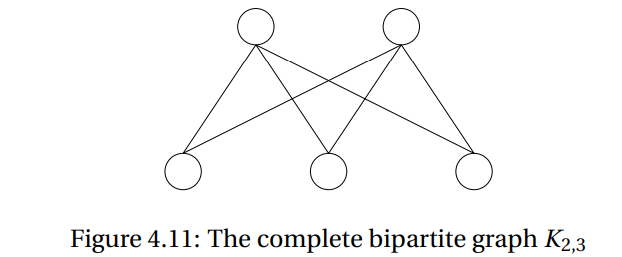
\includegraphics{k2-3.png}
\begin{defn}
    For $n\ge0$, the n-cube is the graph whose vertices are the $\{0,1\}$ strings of length n, and two strings are adjacent if and only if they differ in exactly one position.
\end{defn}
\begin{term}
\begin{itemize}
    \item |V| of n-cube is $2^n$ 
    \item |E| of n-cube is $n\times2^{n-1}$
    \item n-cube is bipartite
    \item n-cube is connected
\end{itemize}
\end{term}
\section{Characterizing bipartite graph}
\begin{lemma}
    An odd cycle is not bipartite.
\end{lemma}
\begin{thm}
    A graph is bipartite if and only if it has no odd cycles.
\end{thm}
\section{Walks and Paths}
\begin{defn}
    A \textbf{Subgraph} of a graph G is a graph whose vertex set is a subset U of $V(G)$ and whose edge set is a subset of those edges of G that have both vertices in U.\\
    spanning subgraph is graph with all vertices but not all edges.\\
    proper subgraph is graph which is not equal to G.
\end{defn}
\begin{thm}
    if there is a walk from vertex x to vertex y in G, then there is a path from x to y
\end{thm}
\begin{corol}
    let x, y, z be vertices of G. If there is a path from x to y in G and a path from y to z, then there is a path from x to z in G. 
\end{corol}
\section{Cycles}
\begin{defn}
    A \textbf{cycle} is a connected graph that is regular of degree 2.
\end{defn}
\begin{defn}
    Alternate \textbf{Path}: The subgraph we get from a cycle by deleting one edge is called a path.
\end{defn}
\begin{term}
    \begin{itemize}
        \item A cycle with n edges is called an n-cycle or a cycle of length n.
        \item Shortest possible cycle in a graph is a 3-cycle.
        \item A spanning cycle in a graph is known as a Hamilton Cycle.
    \end{itemize}
\end{term}
\begin{thm}
    If every vertex in G has degree at least 2, then G contains a cycle.
\end{thm}
\begin{defn}
    The \textbf{girth} of a graph G is the length of the shortest cycle in G.
\end{defn}
\textbf{Connected}
\begin{defn}
    A graph G is \textbf{connected} if, for each two vertices x and y, there is a path from x to y.
\end{defn}
\begin{thm}
    Let G be a graph and let v be a vertex in G. If for each vertex w in G there is path from v to w in G, then G is connected.
\end{thm}
\begin{defn}
    A \textbf{Component} of G is a subgraph C of G such that
    \begin{enumerate}
        \item C is connected
        \item No subgraph of g that properly contains C is connected.
    \end{enumerate}
\end{defn}
\section{Cuts}
\begin{defn}
    Given a graph G and $X \subseteq V(G)$, let $\delta_G(X)$ denote the \textbf{cut} of X in G, meaning the set of edges of G with one endpoint in X and one endpoint in $V(G) \backslash X.$
\end{defn}
\begin{thm}
    A graph G is not connected if and only if there exist a proper subset of V(G) such that the cut induced by X is empty.
\end{thm}
\section{Eularian Circuit}
\begin{defn}
    An \textbf{Eularian Circuit} of a graph G is a closed walk that contains every edge of G exactly once.
\end{defn}
\begin{thm}
    Let G be a connected graph, then G has an Eularian Circuit if and only if every vertex has even degree.
\end{thm}

\begin{defn}
    An edge e of G is a \textbf{Bridge} if G-e ($G \backslash e$) has more components than G
\end{defn}
\begin{lemma}
    if $e = \{x, y\}$ is a bridge of a connected graph, then $g - e(g \backslash e)$ has precisely two components; furthermore x and y are in two different components.
\end{lemma}
\begin{thm}
    An edge e is a bridge of a graph if and only if it is not contained in any cycle of G.
\end{thm}
\begin{corol}
    If there are two distinct paths from vertex u to vertex v in G, then G contains a cycle.
\end{corol}
\begin{term}
    If graph G has no cycles, then each pair of vertices is joined by at most one path.
\end{term}


\section{Tree}
\begin{defn}
    A \textbf{tree} is a connected graph with no cycles.
\end{defn}
\begin{defn}
    A \textbf{forest} is a graph with no cycles.
\end{defn}
\begin{term}
    Every tree is a forest but every forest is not a tree.
\end{term}
\begin{lemma}
    if u and v are vertices in a tree T, then there is a unique u, v-path in T.
\end{lemma}
\begin{lemma}
    Every edge of tree T is a bridge
\end{lemma}
\begin{thm}
    If T is a tree, then 
    \[|E(T)| = |V(T)| - 1\]
\end{thm}
\begin{corol}
    If G is a forest with k components, then
    \[|E(T)| = |V(T)| - k\]
\end{corol}
\begin{defn}
    A \textbf{leaf} in a tree is a vertex of degree 1.
\end{defn}

\begin{thm}
    A tree with at least two vertices has atleast two leaves.
\end{thm}

\begin{term}
    \begin{itemize}
        \item The number of leaves (vertex of degree 1) in a tree is given by 
            \[n_1 = 2 + \sum_{r\ge 3} (r-2)n_r\]
            where r is the degree of vertex, and $n_r$ is the number of vertex of degree r.
        \item A tree that contains a vertex of degree r has at least r vertices of degree one.
    \end{itemize}
\end{term}
\section{Spanning trees}
\begin{defn}
    A spanning subgraph which is also a tree is called a \textbf{spanning tree}.
\end{defn}
\begin{thm}
    A graph G is connected if and only if it has a spanning tree.
\end{thm}
\begin{corol}
    I G is connected with p vertices and $q = p-1$ edges, then G is tree.
\end{corol}

\begin{thm}
    If T is a spanning tree of G and e is an edge not in T, then  $T + e$ contains exactly one cycle C. Moreover if e' is any edge on C, then $T + e - e'$ is also a spanning tree of G. 
\end{thm}

\begin{thm}
    If T is a spanning tree of G and e is an  edge in T, then $T - e$ has 2 components. If e' is in cut induced by one of the components, then T - e + e' is also a spanning tree of G.
\end{thm}
% start from characterizing bipartite graphs

\section{Planar Graphs}
\begin{defn}
    A graph G is \textbf{planar} if it has a drawing in the plane so that its edges intersect only at their ends, and so that no two vertices coincide. The actual drawing is called \textbf{Planar Embedding} of G.
\end{defn}
\begin{term}
    \begin{itemize}
        \item A graph is planar if and only if each of it's component is also planar
        \item A planar embedding partition the plane into connected regions called faces
        \item the outer face in the planar embedding is unbounded.
        \item the subgraph formed by the vertices and edges in a face is called \textbf{boundary} of the face.
        \item Two faces are \textbf{adjacent} if they are incident with a common edge
        \item Boundary Walk
        \item The number of edges in the boundary walk of face f is called the \textbf{degree} of the face f.
        \item A bridge of a planar embedding is always incident with just one face.
        \item A bridge of a planar embedding is always contained in the boundary walk twice, one for each side.
        \item bridge contributes 2 to the degree of the face with which it is incident.
        \item Every edge of a cycle in incident with exactly two faces, and is contained in the boundary walk of each face precisely once.
        \item every edge in a tree is a bridge. so the planar embedding of a tree T has a single face/
        \end{itemize}
\end{term}

\begin{thm}
    if we have a planar embedding of a connected graph G with faces $f_1, \dots, f_s$, then
    \[\sum_{i = 1}^{s}deg(f_i) = 2|E(G)|\]
    Also known as \textbf{Face Shaking Lemma}
\end{thm}

\begin{corol}
    If the connected graph G has a planar embedding with f faces, the average degree of a face in the embedding is $\frac{2|E(G)|}{f}$
\end{corol}

\subsection{Euler's Formula}
\begin{thm}
    Let G be a connected graph with p vertices and q edges. If G has a planar embedding with f faces, then
    \[p-q+f = 2\]
\end{thm}
\begin{term}
    For a given planar graph, the number of faces is always the same, regardless of how you draw it.
\end{term}

\subsection{Nonplanar Graphs}
\begin{lemma}
    If G contains a cycle, then in a planar embedding of G, the boundary of each face contains a cycle
\end{lemma}
\begin{lemma}
    Let G be a planar embedding with p vertices and q edges. If each face of G has degree at least d*, then $(d*-2)q \le d*(p-2)$
\end{lemma}
\begin{thm}
    In a planar graph G with $p \ge 3$ vertices and q edges, we have 
    \[q \le 3p-6\]
\end{thm}
\begin{corol}
    $K_5$ is not planar
\end{corol}
\begin{corol}
    A planar graph has a vertex of degree at most five. \\
    \textbf{this only means atleast one vertex has degree less than equal to 5}
\end{corol}
\begin{thm}
    In a bipartite planar graph G with $p\ge 3$ vertices and q edges, we have 
    \[q \le 2p -4\]
\end{thm}
\begin{lemma}
    $K_{3,3}$ is not planar.
\end{lemma}
\begin{figure}
    \centering
    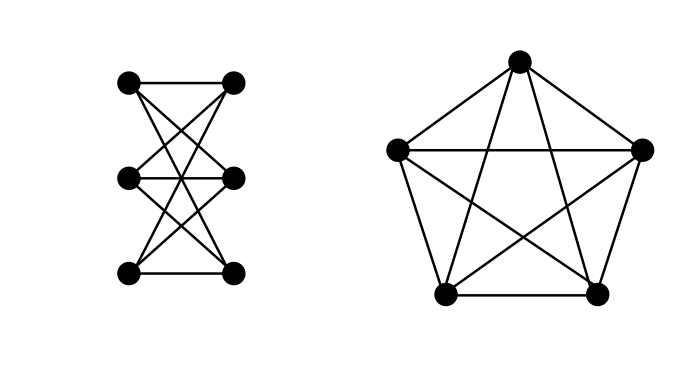
\includegraphics{image.png}
    \caption{$K_{3,3}$ and $K_5$}
    \label{fig:enter-label}
\end{figure}
\subsection{Kuratowski's Theoram}
\begin{defn}
    An \textbf{Edge subdivision} of a graph G, is obtained by applying the following operation, independently, to each edge of G. replace the edge by a path of length 1 or more, if the path has length $m > 1$, then there are $m-1$ new vertices, and $m - 1$ new edges created, if the path has lenght $m = 1$, then the edge is unchanged.
\end{defn}
\begin{thm}
    A graph in not planar if and only if it has a subgraph that is an edge subdivision of $K_5$ or $K_{3,3}$
\end{thm}

\section{Colouring and Planar Graph}
\begin{defn}
    A k-colouring of a graph G, is a function from $V(G)$ to a set of size k (whose elements are called colours), so that adjacent vertices always have different colours. A graph with a k-colouring is called \textbf{k-colourable} graph
\end{defn}
\begin{thm}
    A graph is 2-colourable if and only if it is bipartite.
\end{thm}
\begin{thm}
    $K_n$ is n-colourable, and not k-colourable for any $k < n$
\end{thm}
\begin{thm}
    Every planar graph is all 4,5,6-colourable. \textbf{Read Proof}
\end{thm}

%%%%%%%%%%%%%%%%%%%%%%%%%%%%%%%%%%%%%%%%%%%%%%%%%%%%%%%%%%%%%%%%%%
%Complete the assignment now
\end{document}

%%%%%%%%%%%%%%%%%%%%%%%%%%%%%%%%%%%%%%%%%%%%%%%%%%%%%%%%%%%%%%%%%%
%%%%%%%%%%%%%%%%%%%%%%%%%%%%%%%%%%%%%%%%%%%%%%%%%%%%%%%%%%%%%%%%%%
